\section{Aufbau der Evaluation}
Um die Hypothese zu beweisen oder zu widerlegen, werden drei ausgebildete Designer befragt. Für die Befragung, wird den Probanden zwei verschiedene Szenarien gezeigt, welche zwei der drei Szenarien aus Kapitel \ref{sec:szenarien} abbilden.

Den Probanden werden in einem flowws-Prototyp zwei fertige Graphen innerhalb eine flowws-Prototypen gezeigt, die mit den Szenarien \hyperref[szenario1]{S\#1} und  \hyperref[szenario3]{S\#3} (siehe Kapitel \ref{sec:szenarien}) korrespondieren. Eine genauere Beschreibung der Szenarien inklusive Abbildungen kann in Anhang \ref{anhang:szenario1} und in Anhang \ref{anhang:szenario2} nachgeschlagen werden.

Die Aufgabe der Endnutzer ist es, die verschiedenen Komponenten des Graphen zu identifizieren, ihre Funktion zu deuten und Rückschlüsse über ihr Verhalten zu ziehen. Wenn die Probanden das Verhalten des Graphen antizipieren können, wird im Dialog elaboriert, ob das mentale Modell, dass der Endnutzer gebildet hat, mit dem Konzeptmodell von flowws übereinstimmt. Wenn der Endnutzer das Verhalten des Graphen nicht antizipieren kann, werden im Dialog die Diskrepanzen zwischen dem Konzept- und dem mentalen Modell erörtert. Der Dialog geschieht anhand eines Fragebogens (siehe Anhang \ref{subsec:fragebogen}), der sich auf die \ac{CD} stützt \cite{blackwell2000cognitive}.

Der \textbf{Aufbau} und \textbf{Ablauf} der Evaluation ist wie folgt:
\begin{enumerate}
    \item Der Proband gibt Angaben zu seinen Merkmalen und schätzt sein Fachwissen hinsichtlich \ac{IoT}-Domäne und Programmierung ab (siehe Anhang \ref{subsec:fragebogen}).
    \item Der Proband liest zusammen mit dem Gutachter den Interview Leitfaden (siehe Kapitel \ref{subsec:leitfaden}) durch. Eventuelle Unklarheiten werden hierbei beseitigt. 
    \item Dem Proband werden nacheinander zwei Graphen gezeigt. Nach jedem Graphen wird anhand eines Fragebogens geprüft, ob der Nutzer die Funktionen der einzelnen Komponenten sowie deren Zusammenspiel deuten kann. Es wird als Erfolg gesehen, wenn der Proband von selbst das abgebildete Szenario beschreiben kann, d.h. er hat verstanden, das eine LED von rot zu gelb zu grün wechselt und somit eine Ampel abbildet. 
    \item Nachdem alle zwei Graphen abgearbeitet worden sind, werden generelle Fragen zum Konzeptmodell gestellt. Hierbei werden Fragen verwendet, die sich an den \textit{Cognitive Dimensions} (siehe Kapitel \ref{tab:cognitivedimensions}) nach \cite{blackwell2000cognitive} orientieren. Ziel ist es dabei grundsätzliche Schwächen, Stärken sowie Verbesserungspotential von flowws, zu identifizieren.
\end{enumerate}

Um die Effektivität des \ac{EUD}-Konzeptes möglichst früh zu prüfen, bevor eine vollständige Implementierung vorliegt, wird die hier beschriebene Evaluation auf dem Konzept von flowws in einem frühen Stadium durchgeführt. Die Erstellung eines eigenen Graphen durch den Anwender könnte ergänzend durchgeführt werden, wenn die Implementierung an einer späteren Phase des Projektes abgeschlossen ist. 

\subsection{Prototyp}

\begin{figure}[h]
  \centering
  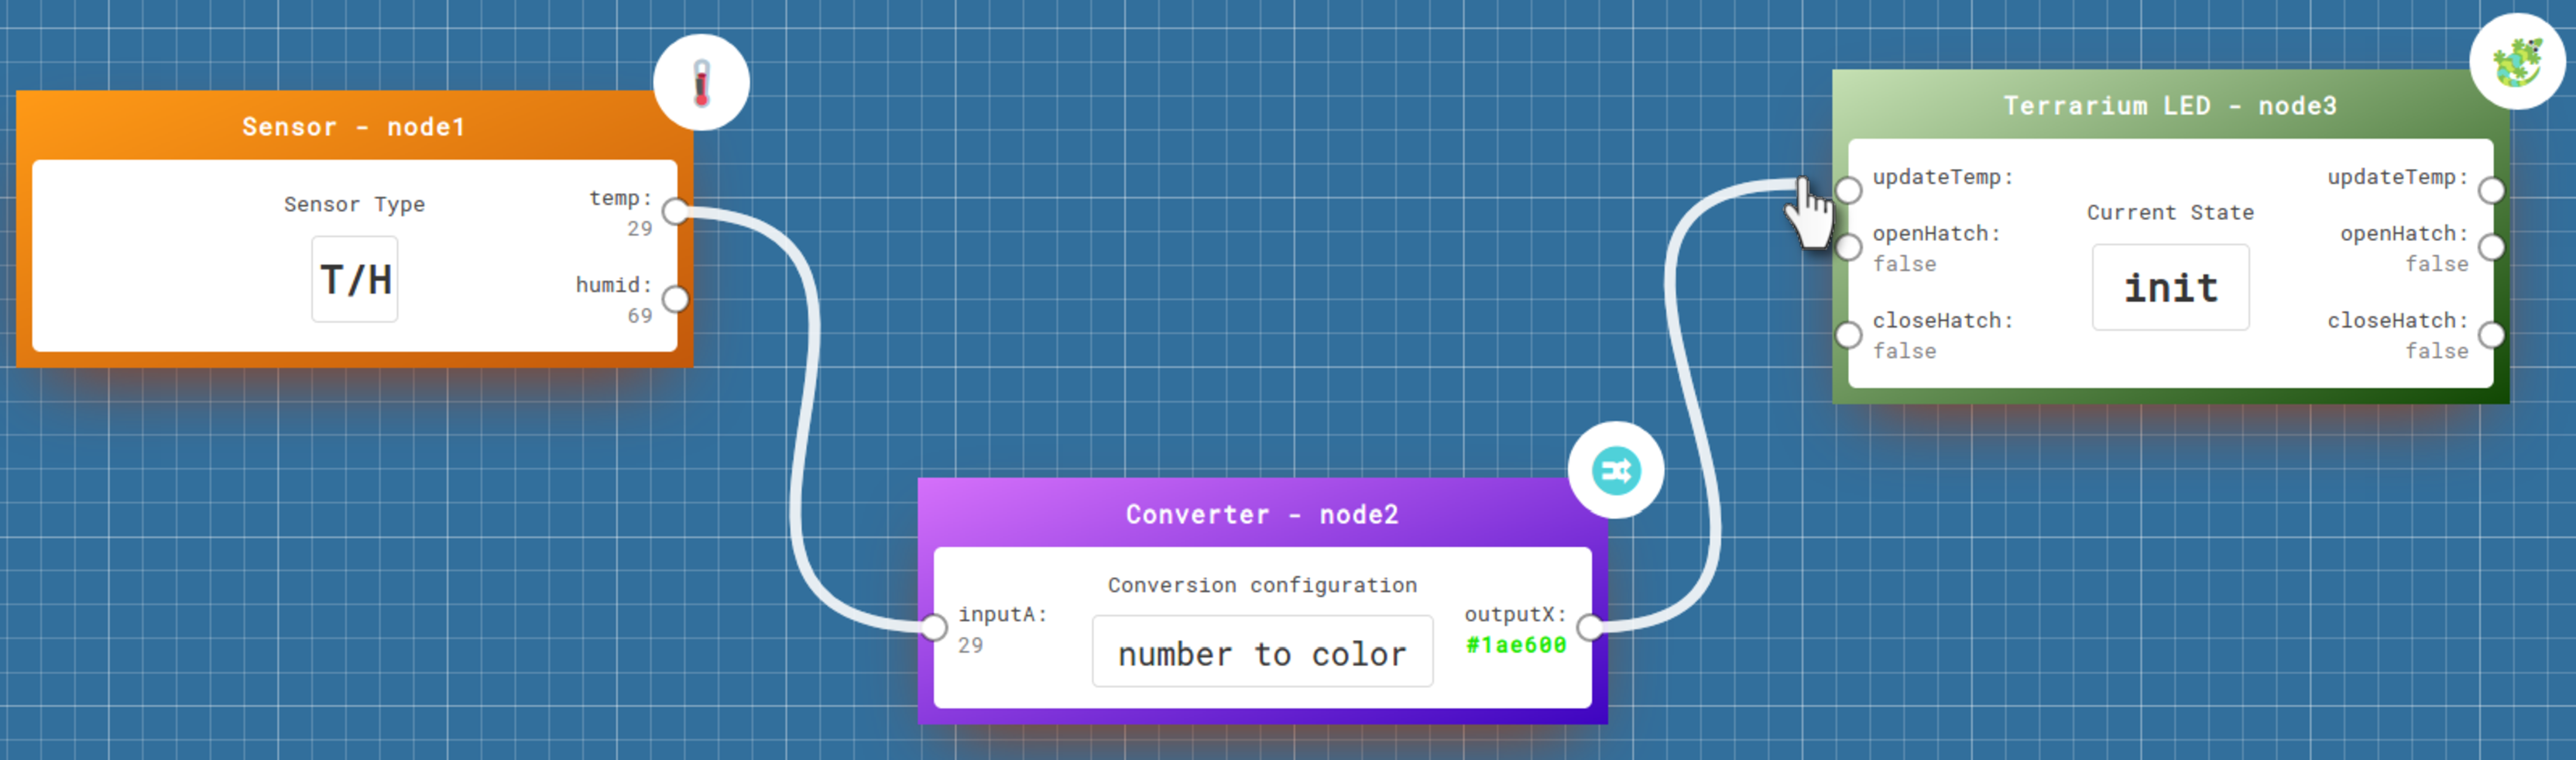
\includegraphics[width=1\textwidth]{bilder/chapter5/screenshotflows.pdf}
  \caption{Screenshot des flowws-Prototyps}
  \label{fig:flowwsprototyp}
\end{figure}

Für die Evaluation wurde im Zuge dieser Thesis eine prototypische Implementierung von flowws erstellt (Beispiel in Abbildung \ref{fig:flowwsprototyp}). Der Prototyp kann die grundlegenden Elemente (Sensor-, Aktor- und Funktionsknoten, Verbindungen) von flowws darstellen und animieren. Darüber hinaus, lassen sich die Elemente miteinander kombinieren und die Signalverarbeitung des Graphen simulieren.

Der Sourcecode wurde als \textit{Webapp} mit dem React-Framework\footnote{\url{https://reactjs.org/} - besucht September 2018} erstellt und steht in einem \textit{Github-Repository}\footnote{\url{https://github.com/chrbrt/flowws} - besucht September 2018} zur freien Verfügung und Erweiterung.
